\documentclass[a4paper, openany]{memoir}

\usepackage[utf8]{inputenc}
\usepackage[T1]{fontenc} 
\usepackage[english]{babel}
\usepackage{amsmath}
\usepackage{amssymb}

\usepackage{booktabs}
\usepackage{fancyhdr}
\usepackage{float}
\usepackage{indentfirst}
\usepackage{graphicx}
\usepackage[linewidth=1pt]{mdframed}
\usepackage{multicol}
\usepackage{fancyvrb}

\pagestyle{fancy}
\fancyhf{}
\fancyhead[LE]{\leftmark}
\fancyhead[RO]{\rightmark}
\fancyhead[RE, LO]{PSD}
\fancyfoot[LE, RO]{\thepage}
\fancyfoot[RE, LO]{Pete Gautam}

\renewcommand{\headrulewidth}{1.5pt}

\chapterstyle{thatcher}
\setcounter{chapter}{14}

\begin{document}
\chapter{Software Architecture Patterns}
Design patterns address design problems at the scale of class interactions. But, they are less suited to addressing large-scale design problems that concern the overall architecture of a software system which may be distributed across many computers and environments. Architectural patterns show reusable solutions to whole system architectural problems.

\section{Model view control}
In user interface design, the information system will typically be responsible for:
\begin{itemize}
    \item storing user data (e.g. images, video, etc.),
    \item presenting different views of the data (e.g. tables, graphs, etc.), and
    \item change in data (e.g. insertion, deletion, updating data).
\end{itemize}
We need an architectural pattern that separates these concerns. An example of this is the model view control (MVC) pattern, given below.
\begin{figure}[H]
    \centering
    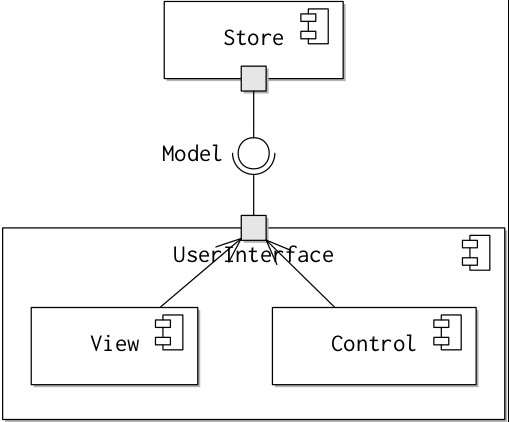
\includegraphics[scale=0.6]{src/14.3 MVC.png}
    \caption{The MVC architectural pattern}
\end{figure}

Architectural patterns are often easier to describe using a component diagram rather than a class diagram. They represent long-lived assemblies in the system rather than the logical organisation of a small number of classes.

The MVC pattern is primarily concerned with the separation of concerns between:
\begin{itemize}
    \item the internal representation of the data held in a store (represented as a model interface),
    \item the different perspectives on the data model (via the view), and
    \item the transformations that can be applied to the data model (via the control).
\end{itemize}
The model interface is shown by the associations with the port on the user interface boundary. The store has no dependency on the other components. 

A key benefit of this approach is that each of the component has a clear responsibility and can be changed without affecting the other components. For example, the components that realise the view and the control can be altered without changing the underlying data representation. Similarly, the implementation of store can be changed independent of the user interface as long as it provides the same model interface. 

Typically, the view and the control components are collated into a single top-level user interface component. This reflects a common situation where the user interface is constructed using a framework/toolkit, such as Swing or Django.

MVC is so prevalent in UI toolkits that it is often not necessary to thinking about arranging the interaction between the user and the system in this way. The design of the framework enforces the conventions. One consequence of this convention is that the view and control are often coupled together. So, changing the control changes how the model is presented to the user in the view, and vice versa.

Beyond system organisation, the MVC pattern leaves considerable flexibility as to how the internal implementation details of the interactions between the components are arranged, e.g.
\begin{itemize}
    \item We can keep some model information in the view. This can be useful if parts of the model don't change very often and repeatedly refreshing the view causes unnecessary cost.
    \item The view can be updated as a result of notifications from the model, or when the view polls the model. Polling can be because of user action or periodic.
    \item The view and control interact directly with the system's user at the system boundary. This may be a human or another software system. The mode of interaction can be textual, graphical, video, etc.
\end{itemize}

\section{Distributed systems}
Distributed systems arose alongside the development of the computing networks and infrastructures such as the Ethernet standards and the Internet. These technologies permitted the different components of the software system to be deployed on physically different computers and communicate according to the standard protocols.

Distributed architectural patterns are concerned with the organisation of services within a distributed system. This is so that the system agrees with a particular design pattern. 

There are several reasons to adopt a distributed system approach.
\begin{itemize}
    \item It might be desirable to access services from different locations because the services provided by the system must be accessible from those locations.
    \item It might be infeasible to store and process data on a single computer.
    \item The system might be composed of many different software components that are managed and implemented by different organisers.
\end{itemize}

There are several reasons why centralising accessed information services could be a good design choice for a distributed software system. The management and organisation of data can be maintained and controlled in a single, consistent structure. The problem of ensuring consistency between multiple copies of the same data is avoided. The approach provides a single, globally known, point of access to the users. Finally, the management of changes to the service functionality can be undertaken in the server rather than in multiple clients.

There are similar benefits to applying the increased data cohesion design principle and the abstraction occurrence design pattern. In both cases, we aim to reduce the cost of managing unnecessary duplications of the data or the software.

\subsection{Client-server architectural pattern}
The client-server pattern embodies this philosophy at an architectural level by collating the management of information services into a centralised server.
\begin{figure}[H]
    \centering
    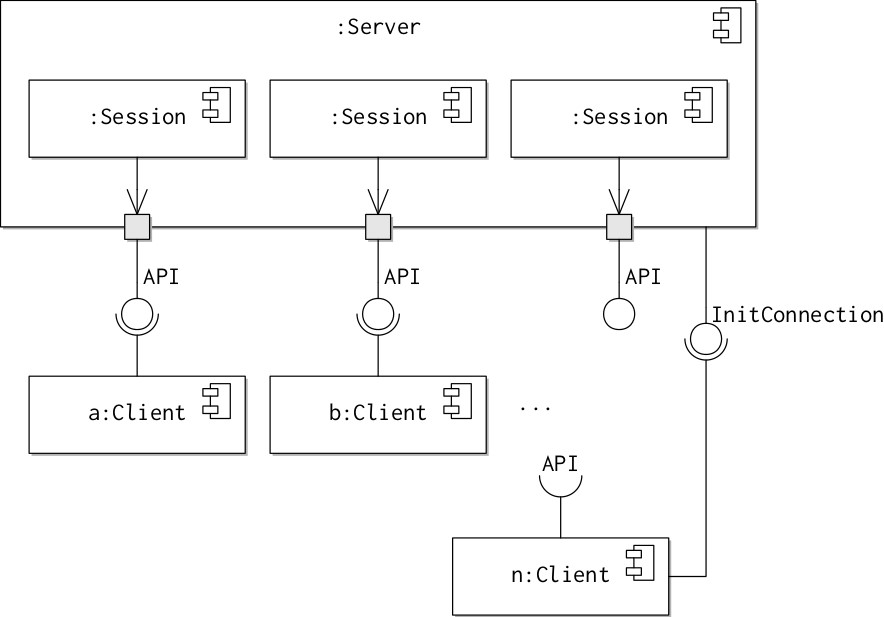
\includegraphics[scale=0.45]{src/14.4 Client server.png}
    \caption{A client-server component diagram}
\end{figure}
\noindent The figure above shows a snapshot of the state of the client-server system, using a component diagram. The components in the diagram are runtime components (denoted by the colon at the start, e.g. \texttt{:Session}) rather than logical components.

The following is how responsibility is divided in the system:
\begin{itemize}
    \item The server is responsible for providing access to the information services it hosts to one of more clients for a component interface.
    \item The server is responsible for ensuring integrity of the information it stores by validating change request from the client.
    \item The client is responsible for presenting the information gathered from the server for the end users by issuing commands to the server. The end users might be people or other software components.
\end{itemize}

Communication between clients and servers is regulated by the definition of the application-level protocol. This describes the legal messages that can pass between the clients and the servers.  In a component-oriented system, the protocol is defined by the server's application programming interface (API). 

In a client-server system, there are 2 interfaces. The first interface is used by the client to indicate that it wishes to establish a new connection with the server. The server exports a second type of interface- the main API. This interface specifies the messages that can be sent once the connection has been established between the client and the server. A separate session component is established each time a client connects to the server. This arrangement allows the server to handle multiple connections with clients simultaneously. The state of the connection, as perceived by the server, is maintained by the session responsible for that connection. 

We see this arrangement in the figure above. The API is provided by the server through a port, but the actual behaviour is realised by session components that are nested inside the server. There is one session component per client, each realising an API interface through a port at a different endpoint. Clients A and B have already established connections and are wired to their respective session components in assembly. 

The unit connection interface is provided by and realised directly by the server. It can be used to create new session components. In the assembly shown, the client N is wired to a connection interface, and the new session has been established. It is ready to be consumed by N's required interface.

There are many examples of client-server architecture and standards in software engineering, such as:
\begin{itemize}
    \item the world wide web,
    \item the subversion version control system,
    \item instant messaging applications, such as Skype, 
    \item the FTP protocol in applications, and
    \item public key infrastructure that supports the implementation of secure commercial communications.
\end{itemize}
\begin{figure}[H]
    \centering
    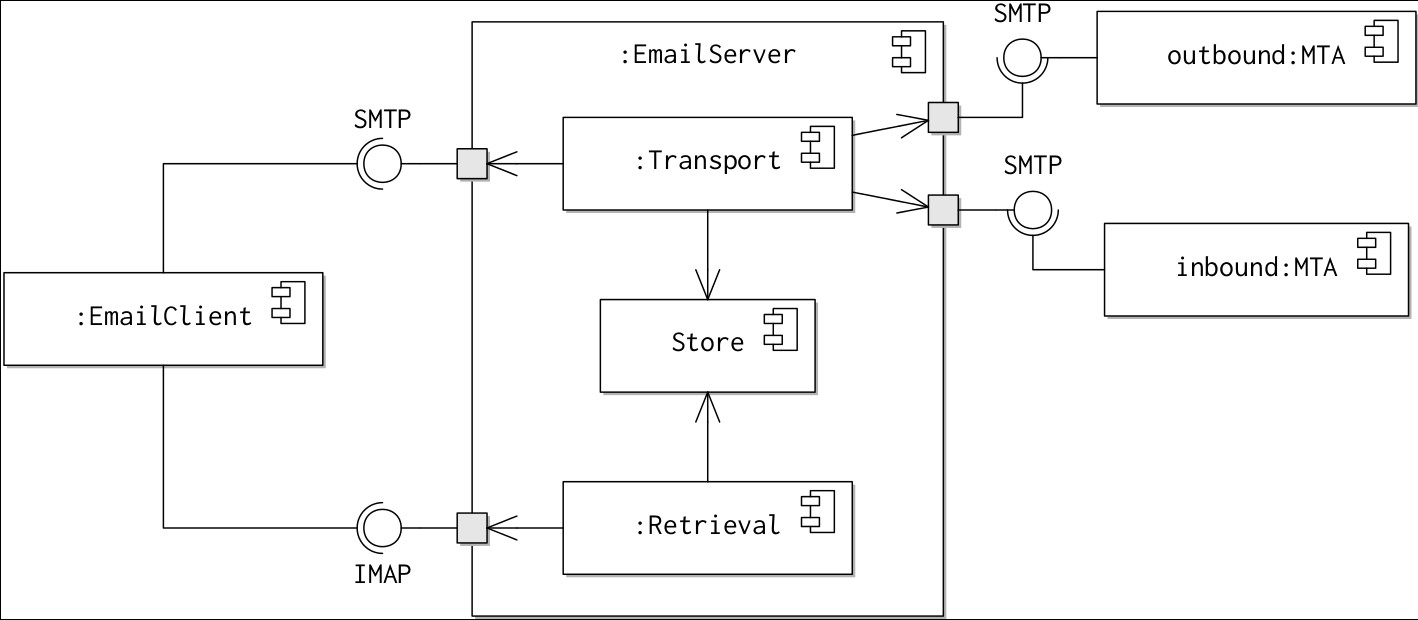
\includegraphics[scale=0.28]{src/14.5 Email component.png}
    \caption{The architecture of a typical email system}
\end{figure}
\noindent The figure above shows the architecture of a typical email system that uses the client-server pattern. The pattern is applied between email clients (e.g. outlook) and email server components. The server provides 2 services:
\begin{itemize}
    \item The retrieval component provides facilities for the client to access and download emails from server via the IMAP interface.
    \item The transport component provides facilities for the client to submit an email for delivery to other users via the SMTP interface.
\end{itemize}
Both the services follow the client-service pattern and implemented by subcomponents. 

The rest of the email architecture is transparent to the client. A separate SMTP interface provided by a remote mail transfer client is used to forward submitted emails to the intended recipients by a relay mechanism. Another  mail transfer agents (MTA) makes use of a third SMTP interface to deliver emails to the server from other users of the system. From the perspective of the external MTA, the email server is just a MTA. 

It makes sense to compose these separate functions (retrieval and delivery) into a single server component. This is because they both rely on the access to the internal email storage component.

There are 2 major styles of client-server pattern.
\begin{itemize}
    \item Thin client architecture is a purist approach to the client-server pattern. In this case, the client is called dumb or terminal because they contain very little program logic. All the information and as much functionality as possible is collected to the server. The client has very little functionality and is only responsible for issuing instructions to the server and displaying results. Even decisions about how to present the data to the clients may be controlled by the server.
    \item Fat client architecture takes the opposite approach. It devolves much more responsibility for information management, validation and processing and storage to clients themselves. This style can be useful because they reduce the amount of communication required between the client and the server; we can cache some information in the client. Some of the processing is delegated to the client. This reduces the computational demands on the server.
\end{itemize}

There is a trade off between thin and fat client architecture. Devolving responsibility to the client reduces load on the server. But, it also risks introducing inconsistencies into the stored data. The clients have to be updated more frequently as software defects are detected.

Fat client architecture has become more popular as processing capabilities of the client environments have improved. This has enabled the development of richer and more interactive user interfaces which are often needed to cache more information.

There are many limitations to the client-server pattern, some of which are listed below.
\begin{itemize}
    \item Communication between servers and clients may suffer from unacceptable latency. That is, it might take too long for the server to receive commands or for the client to receive a response. This could be somewhat mitigated by the client's caching of the information received by the server, like in the case of fat clients.
    \item The scalability of the architecture is bounded by the physical resources available to the server, such as computational power, network bandwidth and memory. This is an inevitable limitation because the server acts as a single point of reference for all the clients. The demands on the server grows as the number of clients increase. This problem is exhibited by the ease with which websites can be disabled by the denial of server (DOS) attack. In the simplest case, the attacker directs as many clients as possible to request the same webpage at the same time.
    \item The single point of reference in the architecture, i.e. the server, is also a single point of failure. So, if the server is disabled, then the entire system ceases to function. This can be mitigated by preparing fallback servers, but this reintroduces the problem of ensuring consistency between multiple copies of the same data items and services.
\end{itemize}

As a consequence, other architectural patterns have been developed to provide a greater scalability and redundancy.

\subsection{Peer-to-peer architecture}
A key problem in client-server architecture is the difficulty of scaling the resources available to the server as the number of clients grow. A fat client architecture is one approach to managing this problem by moving more functionality into the client.

The peer-to-peer architectural pattern extends this approach by moving all services and data in the system into the client themselves. This means that every peer is both a client and a server. The following image illustrates the pattern.
\begin{figure}[H]
    \centering
    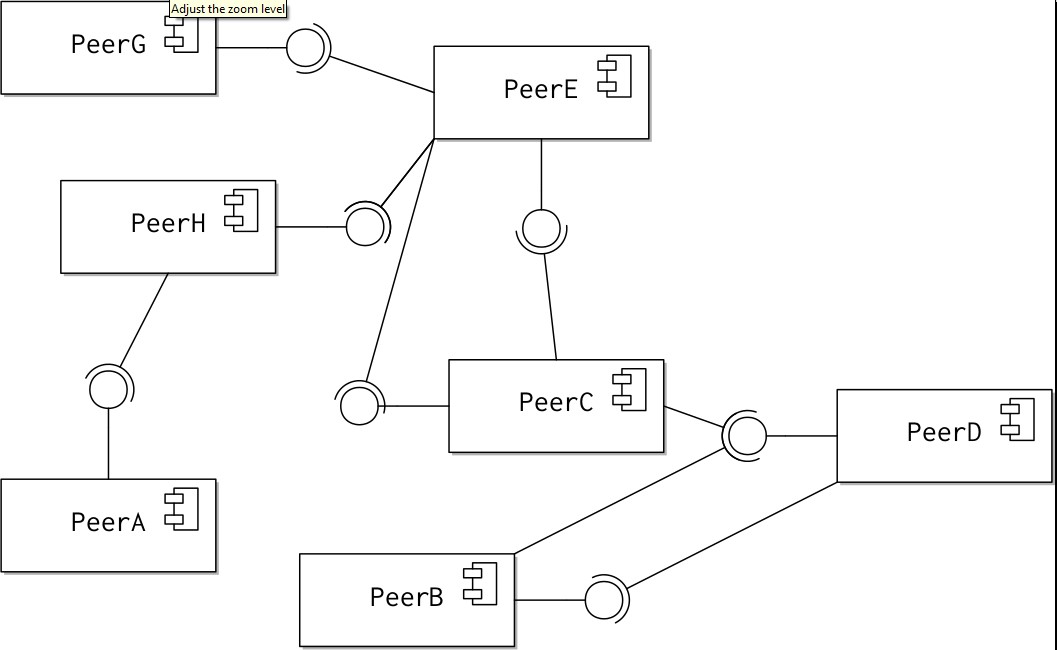
\includegraphics[scale=0.35]{src/14.6 Peer to peer.png}
    \caption{A peer-to-peer architecture.}
\end{figure}

A consequence of this architecture is that the responsibility for hosting and managing services is shared equally amongst all the clients. As the number of clients increases, the demand for resources grow. But, there is also an increase in the number of resources available for the servers, since each peer is both a client and a server.

This means that a peer-to-peer architecture is particularly useful when a system has responsibility for extensive computational processing, or for hosting large amounts of information that isn't possible to host within one single hardware.

The third generation onion rooting project (Tor) is an example of a system that leverages the peer-to-peer architectural pattern. This system is used to support anonymous and untraceable communication between participants on a network that the user suspects is being monitored by an attacker. 

Unlike communication sent directly over an Internet connection, messages in Tor are sent via a random selection of peer nodes in the Tor network. Messages are wrapped in a series of layers of encryption by the sender. Each time a message passes through a Tor node, one layer of encryption is removed. Therefore, the observer of the node cannot match both incoming and outgoing messages. 

Eventually, all the layers of encryption are removed and the message is delivered to the final recipient. As more messages pass through a Tor network, it becomes increasingly more difficult for an observer to work out who the recipient of the message is.

One key challenge in peer-to-peer architecture is service distribution and discovery. The services are distributed to any available and participating node. So, there should be a way to look for other peers offering the same service. Moreover, if anyone can participate in a peer-to-peer system, there should also be a way to determine whether the user can be trusted.

There are several approaches that can be made in a peer-to-peer pattern for peer discovery, including the following.
\begin{itemize}
    \item We can use a globally known registry to record the addresses of peers in the system. Here, a peer first queries the registry to discover the other peers. The registry acts as a super-peer to which all the peers refer first for resource discovery.
    \item We can search across the peer-based network. Here, each peer maintains its registry of known and other peers that have been previously contacted to request the resource. When this happens, the requesting peer also reports the resource it has available. When one peer performs a search for the resource held by another peer, it asks all the peers it knows for the resource. These peers can pass on the request to their known peers, and so on. We continue this until the resource is discovered or the query times out.
    \item We can use a hybrid of the two patterns. In this approach, several registries are deployed. In each registry, there is a list of all the available peers. Each registry attempts to maintain an independent and an up-to-date list of available peers by querying the other registries.
\end{itemize}

All of these styles involve trade offs. Using a globally known registry shares similar limitations to the client-server pattern. That is, if the registry becomes unavailable, then none of the peers will be able to discover the new peers that might have the resources they need. On the other hand, the peer-based search makes no guarantee of finding the required resource. The search might time out before the right period to find the resource is reached. The hybrid approach can mitigate the disadvantages of these approaches, but it cannot eliminate them. Moreover, it introduces a significant additional architectural complexity.

\section{Information Processing Patterns}
Information processing patterns address challenges of efficient information management within the system. It may be used to process large amounts of data or to support effective coordination between components.

We have not yet considered how messages pass between components. We have left this to the component middleware. Also, we assumed that the messages were passing in a synchronous and instantaneous manner. Sometimes, these assumptions are inappropriate for intercommunication, because:
\begin{itemize}
    \item underlying communication channels may be unreliable or subject to delays. This may disrupt the flow of computation in a component.
    \item the client must choose which components will provide the information for a computation because the processing begins. This is because only a single request can be made at a time. So, the minimum amount of time for computation is typically a factor of the number of information requests made rather than any processing or analytical time.
    \item components are forced to request information from other components in a predetermined sequence. This is because they need to wait for a response for each component in turn. However, some applications may not need responses for every request, provided that a sufficient number of responses are being obtained.
    \item the overall system design cannot exploit computational parallelism to improve response time. A component may be unnecessarily idle while it waits for a message to be sent to another component. It could instead be handling messages received from other components in the meantime.
\end{itemize}

Synchronous communication can unnecessarily constrain design flexibility and performance for certain types of computation. For example, consider the component developed to search for the best price for a home insurance premium, given some constraints (e.g. property value, minimum excess, etc.). The components need to contact a large number of insurance providers to request a quotation according to the specification of the customer. The component then chooses the top 5 quotations and presents them to the customer for review.
\begin{figure}[H]
    \centering
    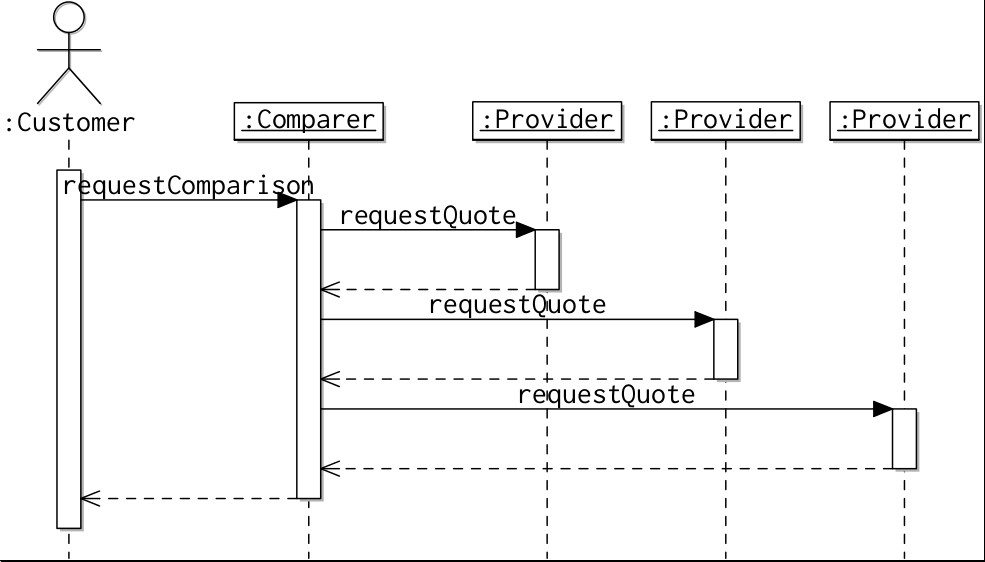
\includegraphics[scale=0.4]{src/14.7 insurance 1.png}
    \caption{Synchronous communication between client and insurance providers.}
\end{figure}

The figure above illustrates the communication between the client and the insurance providers if the client makes its request in a synchronous way. It is a sequence diagram, meaning that time flow is shown vertically and messages between components is shown horizontally. The messages are passed between the clients.

The time taken to identify the best quotation in the example is the sum of the time taken by each of the insurance provider polled. Also, if any provider cannot provide a response, e.g. due to a network failure, then additional time is added to the duration of computation without benefit. In synchronous communication, the component cannot deal with other quotation requests until the first one is completed.

We could do this asynchronously, as shown in the figure below.
\begin{figure}[H]
    \centering
    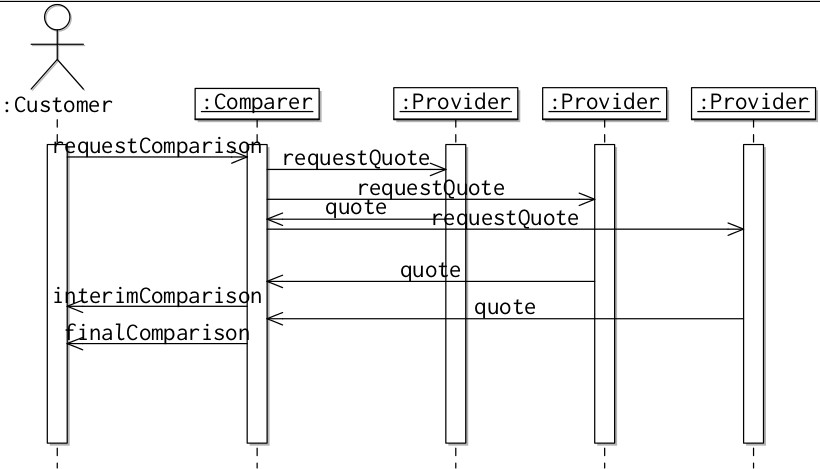
\includegraphics[scale=0.45]{src/14.8 insurance 2.png}
    \caption{Asynchronous communication between client and insurance providers.}
\end{figure}
\noindent Here, the quotation component contacts each of the broker asynchronously. In particular, the client sends a request to each insurance broker without waiting for an immediate reply. Once all the requests are sent, the quotation component waits for a minimum number of insurance providers to respond and sends an initial estimate to the customer. As further quotations arrive, the estimates can be updated.

\subsection{Message-oriented architecture}
The message-oriented architecture pattern provides a basis for general asynchronous communication between components. In the pattern, all communication occurs as discrete messages that pass through the messaging bus. The messaging bus routes messages to the appropriate clients based on a routing policy. 

The pattern is also called:
\begin{itemize}
    \item message-driven pattern since all the internal computation within a component is the result of receiving a message from another component, and
    \item message-broker pattern since a broker is responsible for deciding which components receive a message and acting as a coordinator.
\end{itemize}

The following image illustrates the pattern.
\begin{figure}[H]
    \centering
    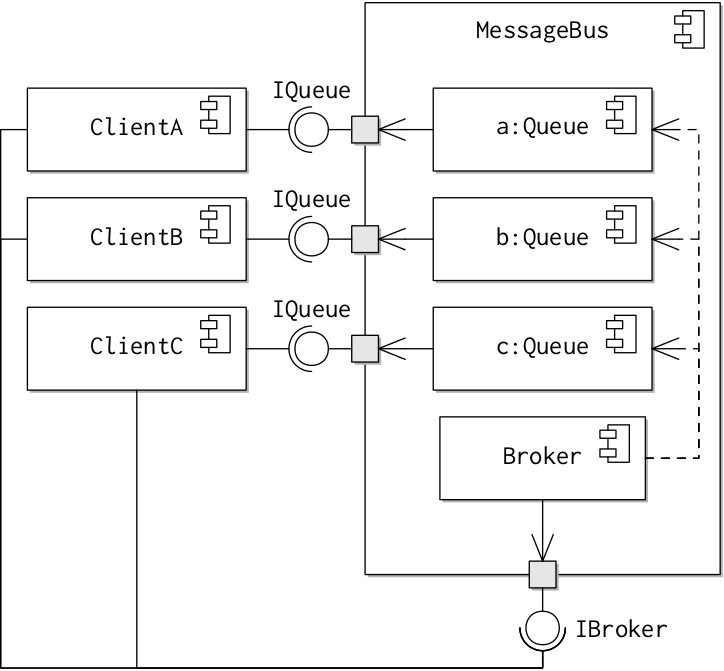
\includegraphics[scale=0.45]{src/14.9 Message.png}
    \caption{The message-oriented architecture.}
\end{figure}
\noindent The message bus is modelled as a single component that provides 2 interfaces:
\begin{itemize}
    \item a broker interface, which is used to send messages to other clients by the bus, and
    \item an IQueue interface, which is used to read messages from the bus that have been sent out specifically to the client by other clients.
\end{itemize}

The use of a standard interface ensures that all messages sent via the bus comply with a pre-described format. This way, every client will know how to parse the structure of the message, even if they are not able to interpret it. 

The image also shows the internal structure of the message bus component. The messages for each client are stored in a Queue component so that there is one queue for each client. Each queue realises the IQueue interface, provided to the appropriate client by the message bus. 

Typically, the client will consume and process messages from the queue as soon as they are available. The queue is used as a buffer when there is a heavy load of messages. The client will also normally block once it has processed all the available messages in the queue.

The client can also  send messages through the broker interface. The interface is realised by the broker subcomponent within a message bus. When a message arrives at the interface, brokers decide which queue the message should be added to. This is normally based on the intended end client.

The broker may not be able to deliver a message, for example, if the queue is full or because the message does not have a valid destination. In this case, the broker is responsible for handling the message. It either drops the message or notifies the client that the message isn't valid (by leaving a message on the sender's queue).

There is considerable flexibility in influencing the behaviour of a message-oriented architecture through mechanisms. There is a relationship between the queues and the clients. Several clients may be connected to the same queue, e.g. if the number of messages added to the queue is typically too much for a single client to handle. Alternatively, a client may listen for messages on several different queues, e.g. a client may maintain separate queues for normal and exception messages.

The policy applied by the broker for distributing messages can be used as well to configure a message-oriented application. The broker may choose between different queues depending on different factors. In particular, the broker may choose the queue because of the intended recipient, because the queue contains the fewest amount of messages, or because of the message type.

Broker pattern is structurally similar to the load-balancing enterprise pattern. But, here the broker decides where to send a request based on load.

For example, consider the stock control system for a large supermarket chain.
\begin{figure}[H]
    \centering
    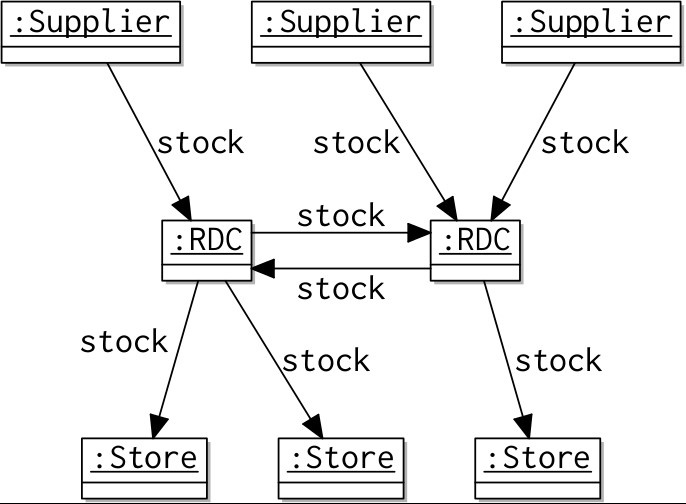
\includegraphics[scale=0.4]{src/14.10 Stock 1.png}
\end{figure}
\noindent The figure above illustrates the flow of stock between different geographical locations. The supermarket chain has a large number of stores, each of which has a limited capacity of holding stocks. The chain maintains a number of regional distribution centers (RDC) for holding larger amounts of stocks on behalf of the stores in the area. 

When the stock of some particular item drops below a certain level in a store, the store management requests additional supplies from the RDC. In turn, the RDC receives stocks directly from the suppliers. In some situations, stocks cannot be sent directly to the appropriate RDC. In that case, the stock is requested from another RDC.

If we use a message-oriented system for the stock control system, we get the following component diagram.
\begin{figure}[H]
    \centering
    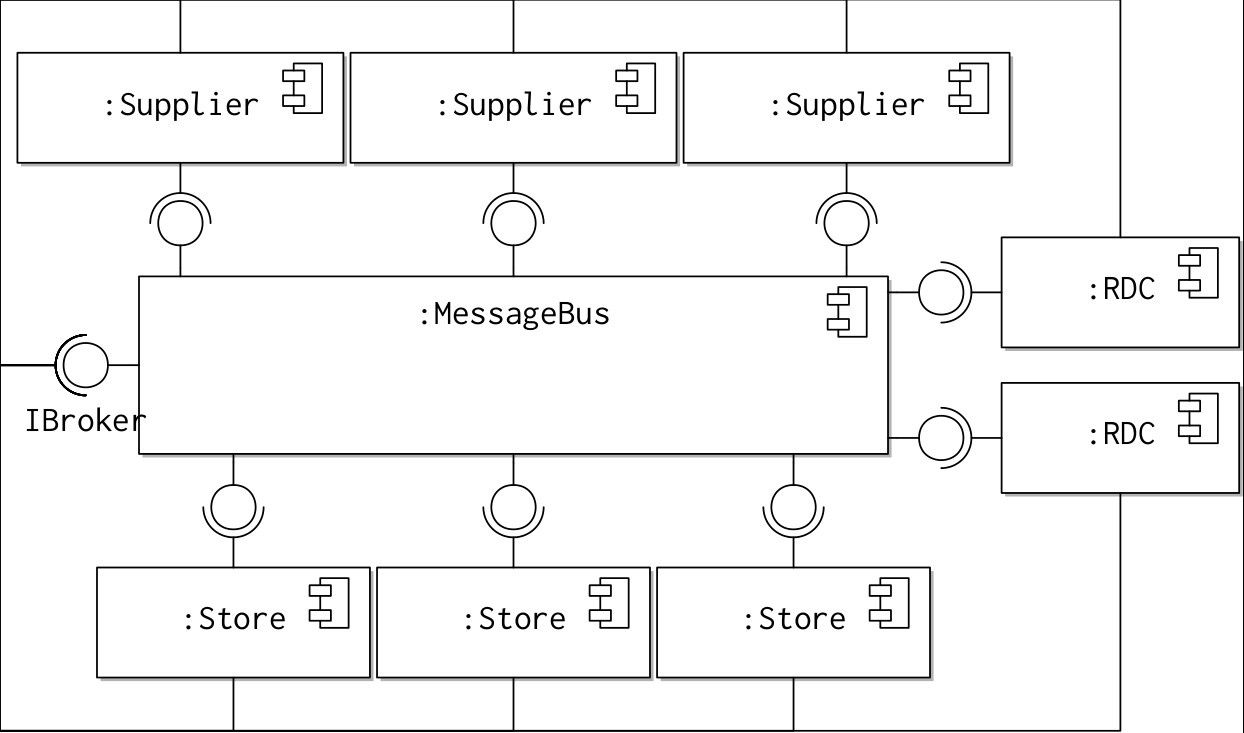
\includegraphics[scale=0.35]{src/14.11 Stock 2.png}
\end{figure}
\noindent The diagram shows the architecture of a message-oriented stock system. Each component has its own queue of messages maintained by the message bus. Each component can send a message to any other component via a broker. In practice, only the following messages are required:
\begin{itemize}
    \item Store to RDC to request for new supplies;
    \item RDC to Suppliers to request for new stock to be delivered;
    \item Suppliers to RDC to notify when the requested products will be delivered;
    \item RDC to RDC to request for stocks to be transferred as available, and to notify when the stock will be delivered.
\end{itemize}

There are several advantages of using a centralised messaging bus to mediate communication:
\begin{itemize}
    \item Communication security is centralised by ensuring all messages pass thro-ugh secured channels on the message bus.
    \item The broker can be configured dynamically to route messages according to the state of the application.
    \item The message bus provides a central location for monitoring intercomponent communication. This is useful for logging interaction between components for debugging or auditing.
    \item This structure also makes it easier to identify bottlenecks and faulty components. This is typically indicated by congested queues.
\end{itemize}

\section{Sequential data processing applications}
Many software applications are required to process large volumes of data by applying a number of transformations between inputs and outputs, e.g.
\begin{itemize}
    \item video and audio media transcoding, where the video gets decoded, reformatted (e.g. resized), and then encoded back.
    \item textual analysis, where a prose is checked for spelling and grammar errors in one language before being translated into another.
    \item inter-bank payment processing, where very large number of small-scale currency transfers must undergo a series of validations before being approved.
    \item processing and synthesising data gathered from scientific instruments. Raw instrument data often needs considerable re-processing and integration before it can be used in analyses. For example, climate data (temperature, pressure, humidity, etc.) is gathered from a variety of sources and using heterogeneous range of instruments.
\end{itemize}

The related applications present several design problems.
\begin{itemize}
    \item Each of the steps in the transformation can take a variable amount of processing time for a given data item. It can result in one or more of the steps becoming a bottleneck, which limits the performance of the application. For example, video data compression may need significant amounts of buffered frame data before it can begin, even though other processes (such as frame resizing) finish more quickly.
    \item Steps may need to be replaced or reordered as the application is adapted to different needs. For example, a generic translation application might need to translate text from different languages. Also, there are different standards for correcting language grammar and punctuation.
    \item It may be desirable to have a convenient means of reusing some functions in combination. In the translation application described above, we can combine a French to English translator with an English to Mandarin translator to produce a French to Mandarin translator.
\end{itemize}

The pipe and filter architectural pattern addresses these design problems by leveraging the homogeneous format of the data being processed. The diagram below illustrates the basic form of the pattern.
\begin{figure}[H]
    \centering
    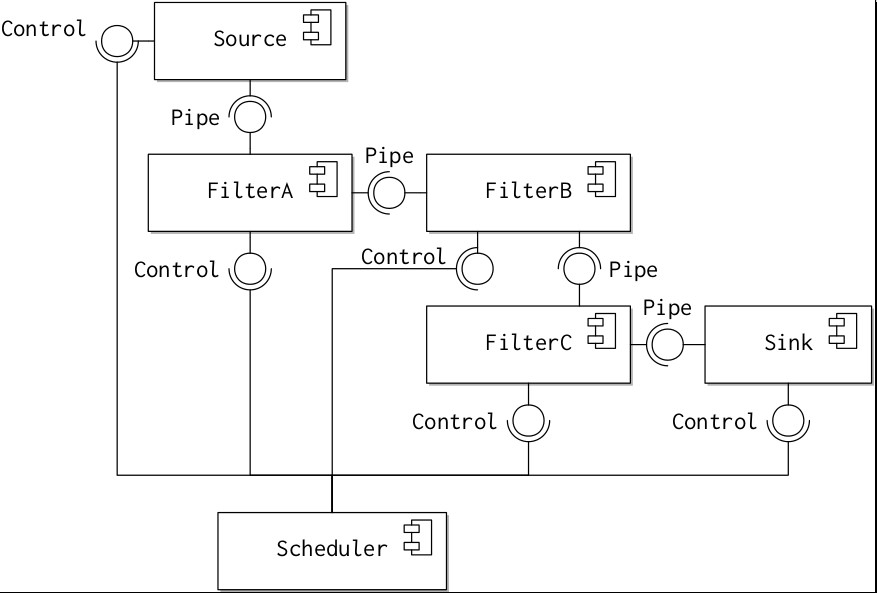
\includegraphics[scale=0.45]{src/14.12 pipe filter.png}
    \caption{The pipe and filter architectural pattern.}
\end{figure}
\noindent Each transformation that must be applied to the data is implemented as a single component called filter. Each filter provides and implements the same interface, called the pipe. The filters are then wired into a single sequential assembly, called the pipeline. Each component obtains its input data from the left, and passes its output to the right.

There are 2 special components on the pipeline:
\begin{itemize}
    \item the data source component provides input on the right, and requires the pipe interface.
    \item the data sink component provides the pipe interface on the right to accept the system's input on the right.
\end{itemize}
Also, a scheduler component is responsible for deciding which of the other components should execute at any given time. The scheduler's job is to manage load between the other components so that no one filter causes a bottleneck in the pipeline. The scheduler controls each component via the control interface.

The pattern specified satisfies the design problems described above. This is because the processor time is allocated to the different filters based on load. This ensures that there is an even flow of data through the pipeline. All of the filters provide and require exactly one pipe interface. So, it can be reordered and composed as necessary.

\subsection{Push or pull data flow}
There are a number of variants to the basic pipe and filter model. Push or pull-driven data flow reflect 2 different controlling processes for moving data to the pipeline. 

The following diagram describes the push model.
\begin{figure}[H]
    \centering
    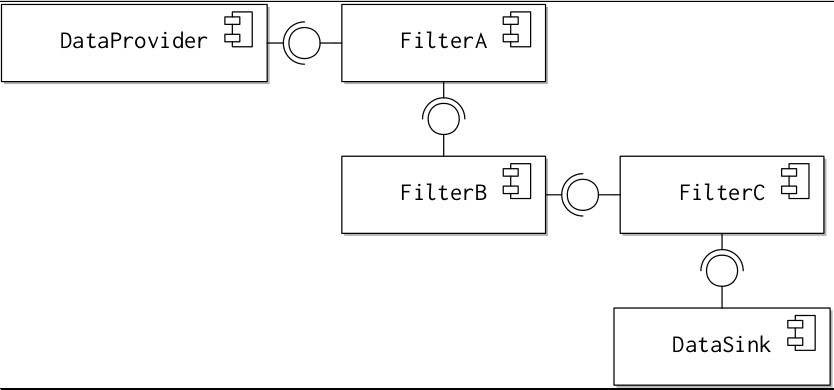
\includegraphics[scale=0.45]{src/14.13 push.png}
    \caption{The push-driven data flow model.}
\end{figure}
\noindent In the push model, data is driven into the system by an active data provider which submits the data to the filter for processing. The data provider will continue to supply data to the filter until the filter is blocked by a full buffer.

In the example above, FilterA will process the data and pass the result onto FilterB, and so on. This process continues until the data is written out to a passive DataSink by the last filter.

The following diagram illustrates the pull model.
\begin{figure}[H]
    \centering
    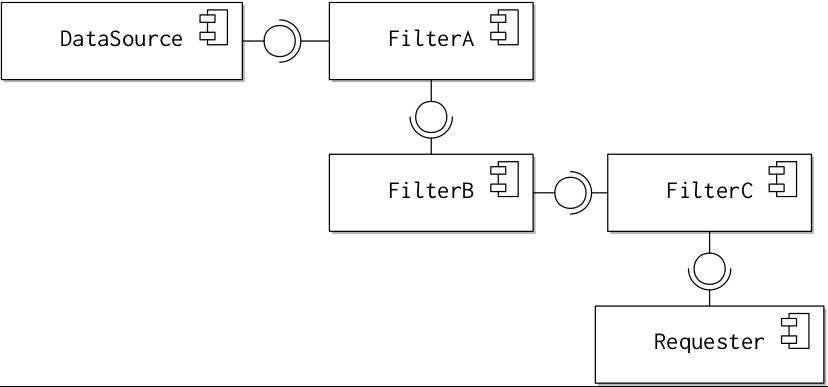
\includegraphics[scale=0.45]{src/14.14 pull.png}
    \caption{The pull-driven data flow model.}
\end{figure}
\noindent The pull model does the reverse of the push model. In this case, a data requester actively polls the last filter FilterC to see for data. Then, FilterC polls FilterB, and so on. This process continues until the last filter polls the DataSource for the data to process. The results are then passed back along the request pipeline. 

The choice of which data model to employ depends on the system for which the application is being used. \begin{itemize}
    \item The push data model is appropriate when the data to be processed is continually generated in an unpredictable/continual way by the provider. This means that the data is fed into the pipeline as and when it becomes available. Multi-media format conversion of an entire media file/continual live stream is a good example of this situation.
    \item A pull data model is appropriate when the data needs to be processed as a result of some external event in the data requester. The requester only initiates the pipeline when it needs the data to be processed. Execution of a scientific experiment that integrates a large collection of diverse datasets and can be a good example of this situation.
\end{itemize}

\subsection{Sequential or concurrent data processing}
Data can be processed in different ways within each filter. The diagram below illustrates the sequential data processing model, using a push-style model.
\begin{figure}[H]
    \centering
    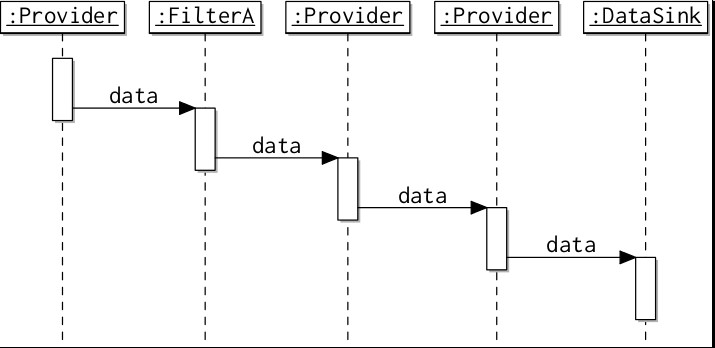
\includegraphics[scale=0.45]{src/14.15 sequential.png}
    \caption{Sequential data processing model}
\end{figure}
\noindent In a sequential pipeline, all the data submitted to the pipeline is processed by each filter in turn, before the data is passed on to the next filter. This means that processing is serialised. The total time taken to process the data is the time taken to process data within each filter.

The diagram below illustrates the concurrent data processing model.
\begin{figure}[H]
    \centering
    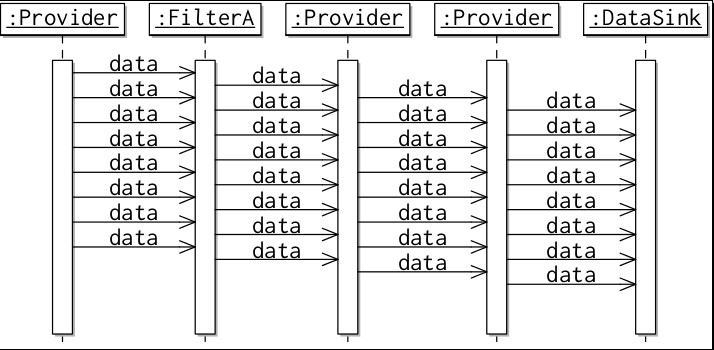
\includegraphics[scale=0.45]{src/14.16 concurrent.png}
    \caption{Concurrent data processing model}
\end{figure}
\noindent In a concurrent pipeline, small amounts of data are fed into the pipeline as soon as they become available. This means that the data sink receives the first blocks of data as soon as they are processed by the last filter.

At first glance, it may seem that the concurrent model is always better. It means that the data arrives at data sink earlier. If the system is distributed in a number of processing nodes, the overall computation should end more quickly. This may be important for certain applications that require a constant stream of data to be written to the data sink, such as video stream.

However, there are many applications where it is better to process larger blocks of data in one go. For example, compression algorithms generally achieve a better compression ratio if they are executed on large blocks of data. Informally, this is because the probability of redundancy increases as the size of the data blocks increases. 

So, there is a trade off between the speed of execution and performance, made in terms of the size of the data block operated on the pipeline.

\subsection{Re-orderable or inter-changeable filters}
Another decision to be made when designing a pipeline architecture is the extent of flexibility that can be permitted in pipeline construction. There are 2 possible variants here- re-orderable and inter-changeable filters.

The most flexible option is to allow the filters to be reordered as desired by the software architect. To enable this arrangement, every single filter must provide and require the same interface. This flexibility means that the overall processing pipeline can be optimised by reordering the processing activity.

For example, in a video-processing algorithm, it is quicker to crop each video frame and then convert it to grayscale, as shown in the diagram below.
\begin{figure}[H]
    \centering
    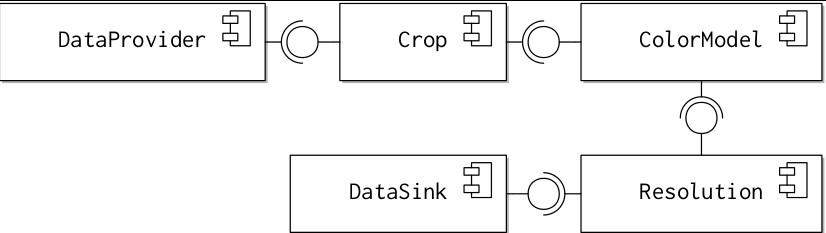
\includegraphics[scale=0.4]{src/14.17 reorderable.png}
\end{figure}
\noindent If we use the reverse configuration, we waste computational time by converting regions of each frame to grayscale that will be removed anyway.

A more restrictive option is to fix the ordering of the filters and only permit the interchange of the filter implementations. In this case, each filter can provide a number of different interfaces. Any filter can be replaced by any other implementation that provides and requires the same interface. 

However, the heterogeneous nature of the filter interfaces means that they cannot generally be reordered. For example, consider an application for converting a scanned image of a page into audible speech in another language, as shown below.
\begin{figure}[H]
    \centering
    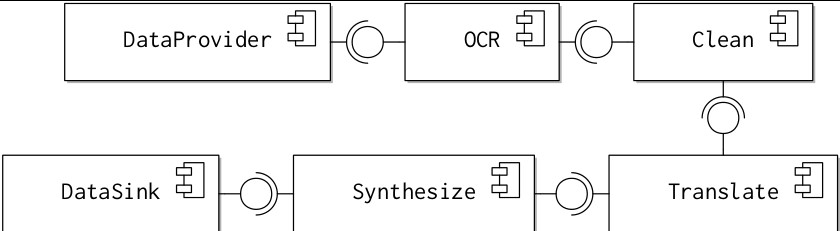
\includegraphics[scale=0.4]{src/14.18 interchangeable.png}
\end{figure}
\noindent The filters of the system might be: optical character recognition (OCR), spelling and grammar check, text translation and speech synthesiser. These components cannot be reordered, and each filter requires a different form of input data type. However, the implementation of each component can be swapped around as required. This is inter-changeable filter model.

Again, it is possible to compromise between the two architectures so that some parts of the pipeline can be reordered and others require set sequences of filter types.

A final variant is to allow the use of branching filters to a pipeline, as shown below.
\begin{figure}[H]
    \centering
    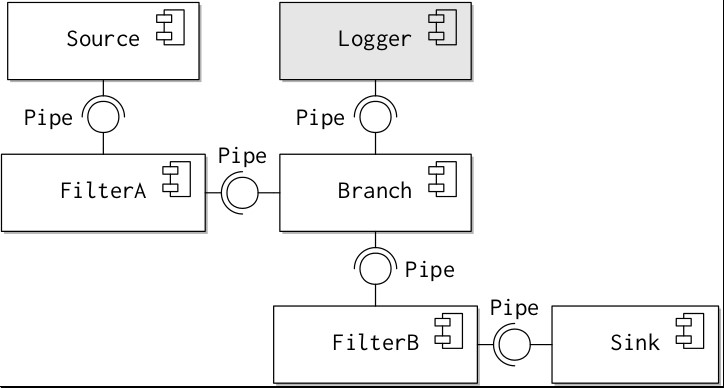
\includegraphics[scale=0.45]{src/14.19 branching filters.png}
\end{figure}
\noindent The branching filter can do one of 2 things to incoming data:
\begin{itemize}
    \item replicate the data stream to the outgoing filters, or
    \item filter each data item into one of the outgoing branches.
\end{itemize}

Branches can be useful in pipelines for several reasons:
\begin{itemize}
    \item We can perform ancillary functions on exact copies of data, e.g. logging intermediate versions of the dataset during computation,  debugging for verification, etc. This may mean that the functions do not have to be built into filters themselves.
    \item We can apply two different transformations to some incoming data source simultaneously, e.g. a video stream might need to be encoded for high and low-quality distribution.
    \item We can separate data items in terms of different categories for alternative processing. A data stream might contain words in 2 different languages that need to be separated and processed differently, for example.
\end{itemize}

\section{Plugin architecture}
Sometimes, it can be difficult to predict all the required functionalities for an application beyond a core set of features. This may be for the following reasons:
\begin{itemize}
    \item It is anticipated that new features may need to be added over time as requirements change. 
    \item Different users of application may have different requirements, and providing all the required features to all users would result in an overly complex system and user interface.
    \item It is anticipated that some users will want to develop their own functionality for the system, and tailoring each of the features for their own personal needs.
    \item The application will run on different platforms, some of which will not be able to support all of the application's functionality and will have to do it in different ways.
\end{itemize}

Plugin architecture provides a flexible mechanism for extending the functionality of the software system. In the pattern, an application is able to dynamically search for and load components that contain additional functionality into the main system.

The diagram below illustrates the key components in the plugin architectural pattern.
\begin{figure}[H]
    \centering
    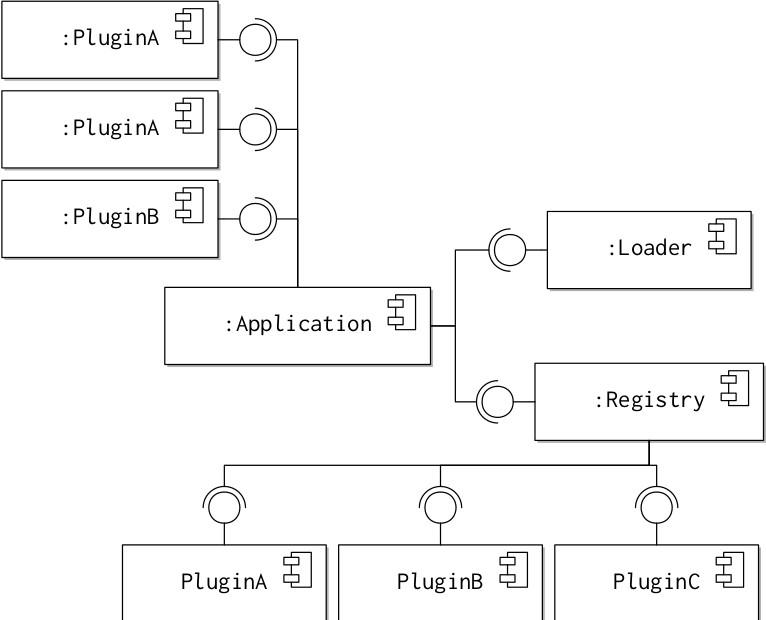
\includegraphics[scale=0.45]{src/14.20 plugin.png}
    \caption{The plugin architecture.}
\end{figure}
\noindent The main  component in the architecture is the registry that stores the specification of all plugins available to the system. 

A plugin component normally provides a standard interface that compiles with the requirements of the plugin architecture. This can provide:
\begin{itemize}
    \item details on how to instantiate the plugin in an application,
    \item details on how the component can be used in the architecture.
\end{itemize}
The main application can query the registry for available specifications of a particular type. When an appropriate plugin is located, a load of component is used to instantiate and configure the component for use by the main application, using the specification supplied by the registry. The plugin's functionality can then be accessed via the specified interfaces just like any other component in the system.

The plugin architecture is similar to a software framework that exhibits hooks and slots. However, the purpose of the two is quite different. 
\begin{itemize}
    \item A software framework is not an application. It is a collection of utilities, libraries and infrastructures for building applications in a particular architectural style or for a particular purpose.
    \item A plugin architecture is a complete application by itself. The plugins provide useful extensions to that core functionality.
\end{itemize}

The diagram above distinguishes between runtime components (which have been instantiated by the loader) and the logical components (which have been stored within the registry). The logical components are the descriptions and the specifications of the components, whereas the runtime components are the actual loaded and installed runtime representations of the same components. It allows us to have duplicates of the same component loaded in the application.

A plugin architecture should be used for extending the functionality of a specific application, and not for building the whole application. Consequently, the range of ways in which a plugin can extend the application's functionality and purpose should be carefully constrained. 

An application that is built purely from plugins is in danger of exhibiting the inner platform effect. This means that the developers are in danger of reinventing the application, effectively as its own programming language, rather than using the existing, underlying programming language and framework to design the application's functionality.

In summary, software architecture helps developers to reason about the high-level structure and key components of a software system.



\end{document}